\chapter{Method}
\label{ch:method}


This chapter describes the implemented monocular thermal-inertial odometry (TIO) pipeline concretely, from thermal preprocessing through the feature front-end and the MSCKF back-end, to initialisation and the evaluation framework.

\section{System Overview}
\label{sec:m_overview}
The implemented system is a monocular thermal-inertial odometry pipeline that consumes a stream of images and inertial measurements and produces a metric trajectory estimate. It is organised into three deliberately decoupled layers. The \emph{preprocessing} layer turns each raw high-bit-depth frame into an $8$-bit image suitable for the front-end. The \emph{front-end} detects and tracks features across frames, producing feature tracks---sequences of image observations of the same scene point---after an outlier-rejection stage. The \emph{back-end} is the MSCKF of Section~\ref{sec:bg_msckf}, which propagates the state with the inertial measurements and updates it with the feature tracks. Images and inertial samples are associated by timestamp, with the filter propagated over the inertial samples that fall between consecutive frames. The full pipeline is shown in Figures~\ref{fig:pipeline_clahe_norm} and~\ref{fig:pipeline_norm_clahe} in Section~\ref{sec:m_preproc}, which differ only in the ordering of the two preprocessing operators examined in that section.

The three layers communicate through narrow interfaces---an $8$-bit image, a list of feature tracks, and the filter state---so that each can be modified or replaced without touching the others. This modularity is deliberate: it lets the front-end be switched between KLT and ORB, the preprocessing operators and their ordering be varied, and the back-end parameters be tuned, all independently, which is precisely what the sensitivity study of Chapter~\ref{ch:results_and_discussion} exploits. The pipeline is implemented in Python, using OpenCV for the image operations and feature front-ends and NumPy/SciPy for the filter linear algebra. Only a single (left) camera is used, and the system is run offline on recorded data; a deployed instance would output the same raw metric trajectory online. The remaining sections describe each layer in turn: thermal preprocessing (Section~\ref{sec:m_preproc}), the feature front-end (Section~\ref{sec:m_frontend}), the MSCKF back-end (Section~\ref{sec:m_backend}), initialisation (Section~\ref{sec:m_init}), zero-velocity updates (Section~\ref{sec:m_zupt}), the filter and front-end parameters (Section~\ref{sec:m_params}), and the evaluation framework (Section~\ref{sec:m_eval}).

\section{Thermal Preprocessing}
\label{sec:m_preproc}
Each raw thermal frame passes through a fixed chain of operators before reaching the front-end: undistortion, Gaussian denoising, and---in one of two orderings---contrast enhancement and $8$-bit normalisation. Both orderings were implemented; the full pipeline is shown for each in Figures~\ref{fig:pipeline_clahe_norm} and~\ref{fig:pipeline_norm_clahe}.

\begin{figure}[htbp]
    \centering
    \begin{minipage}{0.45\linewidth}
        \centering
        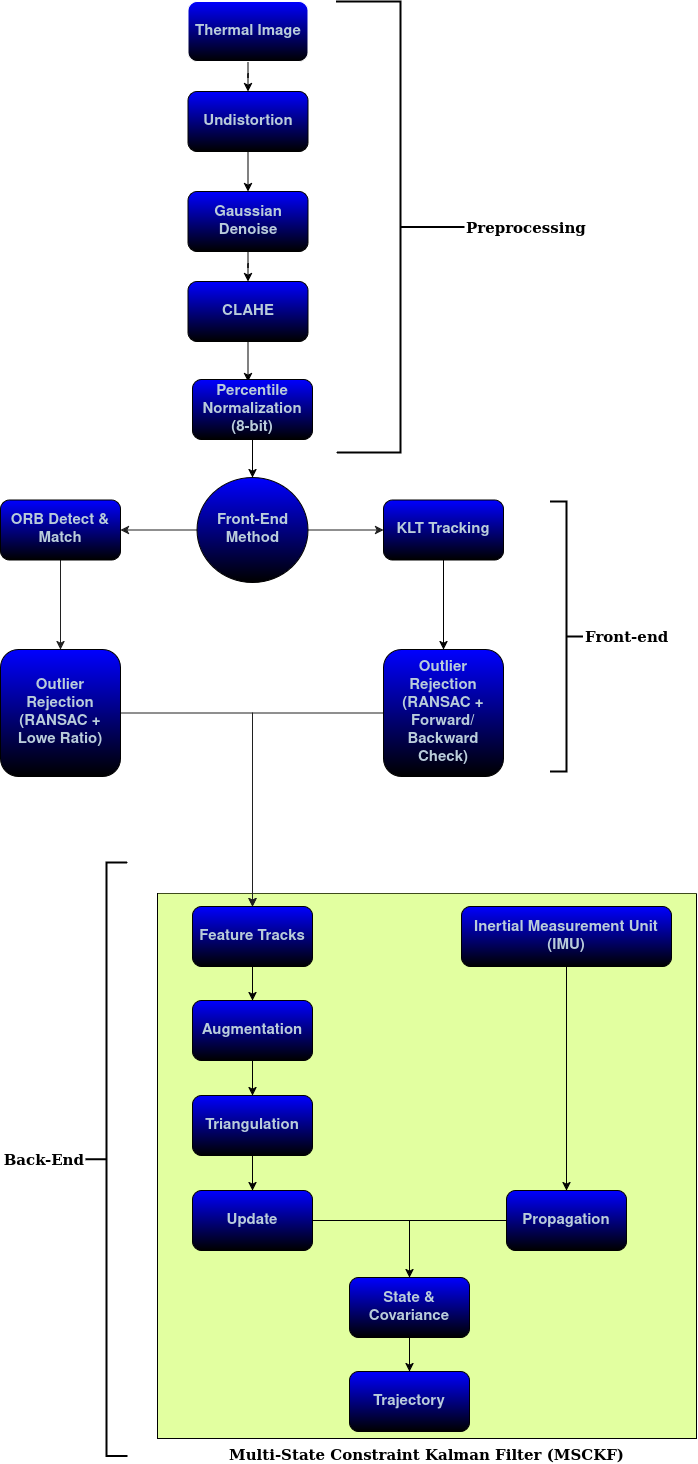
\includegraphics[width=\linewidth]{Figures/clahe_norm.png}
        \caption{MSCKF pipeline---CLAHE before normalisation.}
        \label{fig:pipeline_clahe_norm}
    \end{minipage}
    \hfill
    \begin{minipage}{0.45\linewidth}
        \centering
        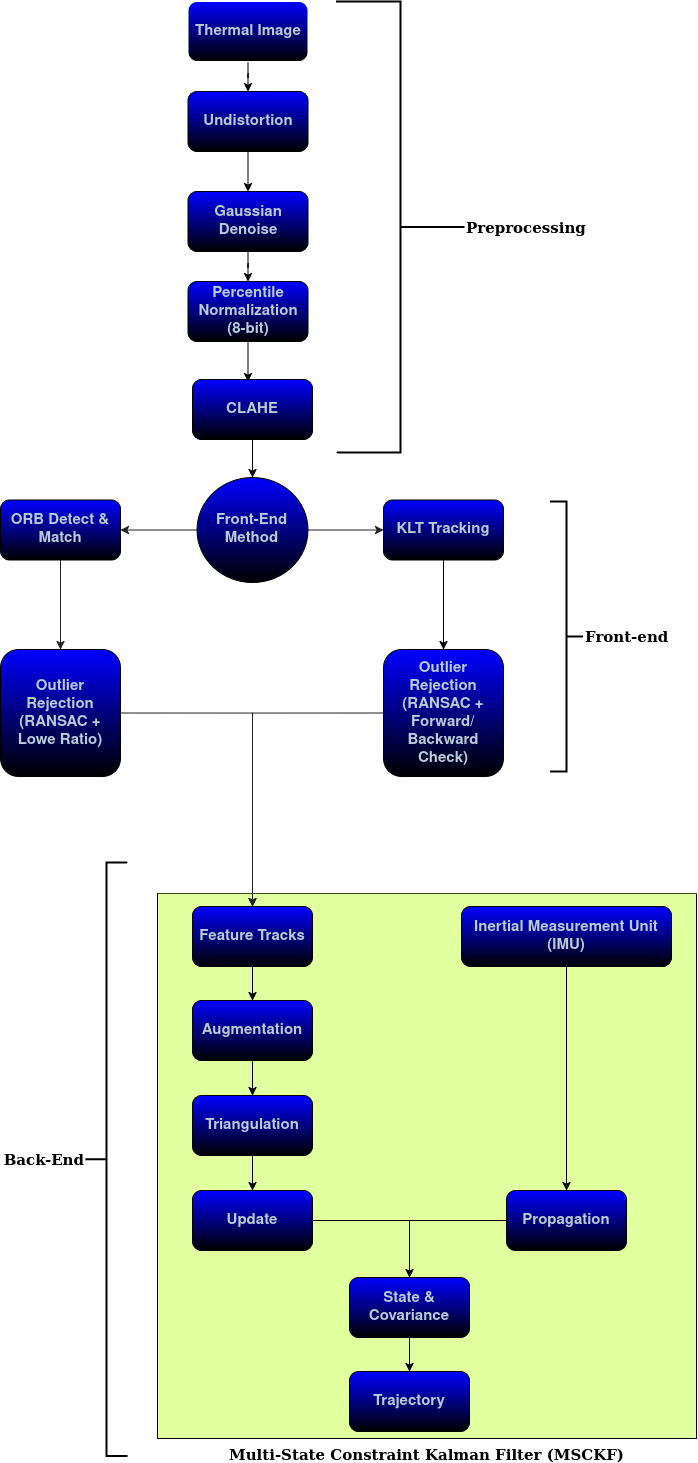
\includegraphics[width=\linewidth]{Figures/norm_clahe.png}
        \caption{MSCKF pipeline---CLAHE after normalisation.}
        \label{fig:pipeline_norm_clahe}
    \end{minipage}
\end{figure}

\textbf{Undistortion.} Raw thermal frames exhibit lens distortion whose magnitude depends on the specific camera and lens, which would otherwise make the apparent motion of a feature inconsistent from one frame to the next. Each frame is undistorted with a precomputed remap look-up table built from the calibrated intrinsics $\mathbf{K}$ and distortion coefficients $\mathbf{D}$ (a plumb-bob or fisheye model, depending on the dataset), so that feature motion reflects camera motion alone. The remap keeps $\mathbf{K}$ unchanged, so tracked pixels can be mapped directly to normalised bearings with $\mathbf{K}^{-1}$ in the measurement model of Section~\ref{sec:bg_measurement}.

\textbf{Denoising.} Thermal sensors exhibit per-pixel speckle noise. A Gaussian blur (kernel size $3\times3$) is applied before contrast enhancement, so that the enhancement step does not amplify this noise into spurious gradients that would otherwise be picked up as false corners by the front-end.

\textbf{Contrast enhancement and normalisation.} The sensor's native $14$- or $16$-bit radiometric output must be mapped to the $8$-bit range expected by the front-end, and its native contrast is low. Contrast-Limited Adaptive Histogram Equalisation (CLAHE) is applied with a clip limit of $3.0$ on an $8\times8$ tile grid, and the $8$-bit mapping is obtained by a per-frame percentile normalisation (clipping to the $2$nd and $98$th percentile of the frame). These two operators do not commute: CLAHE's clip limit is defined relative to the histogram it operates on, so applying it before or after the bit-depth reduction changes its effect. Both orderings were therefore implemented, as separate, otherwise identical preprocessing paths, and compared empirically; the comparison and the ordering adopted for the final results are reported in Section~\ref{sec:r_preproc}. Figure~\ref{fig:m_preproc_chain} illustrates the two intensity-mapping stages of this chain---normalisation and CLAHE---on a representative frame; the undistortion and Gaussian denoising applied beforehand are not perceptible at this scale and are omitted.
\vspace{10mm}
\begin{figure}[htbp]
    \centering
    \includegraphics[width=\linewidth]{Figures/fig_preproc_chain.png}
    \caption{The intensity-mapping stages of the adopted Norm$\rightarrow$CLAHE preprocessing chain on one ROVTIO frame; the undistortion and $3\times3$ Gaussian denoising applied first are imperceptible on the raw frame and are omitted here. The raw radiometric values occupy only a thin slice of the 16-bit range (here $\approx3150$--$3327$ of $0$--$65535$), so shown on the full scale the frame reads as nearly flat and dark (left)---which is precisely why an 8-bit mapping is needed. Per-frame percentile ($2$--$98\%$) normalisation stretches that slice across the 8-bit range (centre), recovering the global dynamic range, and CLAHE (clip $3.0$, $8\times8$) then adds the local contrast and edge detail the front-end relies on (right).}
    \label{fig:m_preproc_chain}
\end{figure}

\section{Feature Front-End}
\label{sec:m_frontend}
Two front-end variants are implemented and compared in this thesis: Kanade--Lucas--Tomasi (KLT) optical-flow tracking and ORB detection and descriptor matching. Both produce the same output---a set of feature tracks, each a sequence of pixel observations of one scene point across consecutive frames---so either can be fed to the back-end of Section~\ref{sec:m_backend} without modification. Both variants share a geometric outlier-rejection stage---a maximum-displacement gate and a RANSAC fundamental-matrix test---but each additionally applies a check specific to its matching mechanism: a forward--backward consistency check for KLT and Lowe's ratio test for ORB, as detailed in the subsections below. The gates specific to triangulation---parallax, depth, and the $\chi^2$ consistency test---are deferred to the back-end, where they act once a track's observations are used in an update.

The fundamental matrix is used only for geometric verification of correspondences, not for pose recovery, which comes from the IMU--MSCKF fusion; a calibration-free fundamental-matrix fit is therefore sufficient and no essential-matrix decomposition is performed. The eight-point fundamental-matrix estimate degenerates under low parallax, pure rotation, or planar scenes, where a near-static baseline makes the epipolar geometry ill-defined and the test can admit spurious inliers; in this regime the parallax and $\chi^2$ gates of the back-end (Section~\ref{sec:m_backend}) act as the primary safeguard.

\subsection{Kanade--Lucas--Tomasi Tracking}
\label{sec:m_klt}
KLT tracking follows a feature by directly matching local pixel intensities rather than a descriptor. Features are first located as Shi--Tomasi corners~\cite{Shi_1994}: image points with a strong intensity gradient in two directions, and therefore well localised. Each corner is then followed from one frame to the next with pyramidal Lucas--Kanade optical flow~\cite{Lucas_1981}, which estimates, for a small window centred on the point, the sub-pixel displacement that best aligns the window's intensity pattern between the two frames; a coarse-to-fine image pyramid allows this to accommodate larger inter-frame motions than a single-resolution search.

Because thermal imagery often has low geometric texture, few strong corners may be available; where they are, KLT is well suited to tracking them since it matches intensities directly and does not depend on a repeatable descriptor, unlike ORB's binary descriptor, which is more sensitive to the modality's contrast and noise. Its corresponding weakness is that it relies on brightness constancy---the assumption that a physical point's apparent intensity is unchanged between frames---which the radiometric instability of thermal sensors (Section~\ref{sec:bg_thermal}) can violate.

Two checks reject unreliable tracks before they reach the back-end. A forward--backward consistency check tracks each point forward from frame $n-1$ to $n$ and then backward from $n$ to $n-1$; if the round trip does not return close to the original pixel, the correspondence is discarded. A maximum-displacement gate then rejects any correspondence whose pixel motion exceeds a fixed bound. The surviving correspondences across the whole frame are finally fitted jointly to a fundamental-matrix model with RANSAC~\cite{Fischler_1981}; points inconsistent with this common two-view geometry are rejected as outliers, rather than being judged individually. Because KLT carries no descriptor, a track that is lost cannot be re-acquired: whenever the number of active tracks falls below a set threshold, new Shi--Tomasi corners are detected in the regions not already covered by a track, replenishing the set. The surviving tracks are passed to the back-end.

\subsection{ORB Detection and Matching}
\label{sec:m_orb}
ORB tracking instead re-identifies features by descriptor matching rather than following pixel intensities. In each frame, FAST corners are detected and a $256$-bit binary BRIEF descriptor~\cite{Rublee_2011} is computed for each; detection is performed on a grid of cells covering the image, retaining only the strongest corners per cell, so that features are not concentrated in the highest-contrast regions of the frame at the expense of coverage elsewhere.

Correspondences with the previous frame's tracked descriptors are established by Hamming-distance matching. For robustness, matching is run in both directions---from the previous frame's descriptors to the current frame's and back---and a correspondence is kept only if it is each other's nearest neighbour in both directions (mutual nearest-neighbour consistency) and if its distance is sufficiently smaller than that of the second-nearest candidate (Lowe's ratio test), which rejects ambiguous matches in repetitive or low-texture regions. As with KLT, the surviving correspondences are then passed through the same maximum-displacement gate and a joint RANSAC fundamental-matrix test before being accepted as tracks.

Because matching is descriptor-based rather than sequential, ORB can in principle re-associate a feature after a brief loss without re-detection. This comes at the cost of depending on the descriptor's repeatability, which the low native contrast and higher noise of thermal imagery (Section~\ref{sec:bg_thermal}) can undermine, making correct matches harder to distinguish from incorrect ones by Hamming distance alone.

\section{MSCKF Back-End}
\label{sec:m_backend}
The back-end implements the MSCKF of Section~\ref{sec:bg_msckf} with the concrete choices described here. The inertial state is propagated between images by the prediction of Section~\ref{sec:bg_imu_kin}, and the sliding window is bounded to a fixed number of camera poses $N_{\max}$.

\textbf{State augmentation.} When an image is received, the current camera pose is computed from the inertial state and the fixed extrinsics, $\mathbf{R}_{C}^{W} = \mathbf{R}_{I}^{W}\,\mathbf{R}_{C}^{I}$ and $\mathbf{p}_{C}^{W} = \mathbf{p}_{I}^{W} + \mathbf{R}_{I}^{W}\,\mathbf{p}_{C}^{I}$, and appended to the state. This is a deterministic cloning of the current pose rather than a prediction or an update: it enlarges the dimension of the state and covariance without injecting any process noise, so the estimate's uncertainty is not increased, only extended to the new pose. The new block is formed through the augmentation Jacobian, whose key coupling term is the lever-arm block $-\mathbf{R}_{I}^{W}\lfloor\mathbf{p}_{C}^{I}\rfloor_{\times}$, which expresses how the new camera position depends on the IMU attitude error.

\textbf{Measurement update.} A feature is used to update the filter only once it can no longer be tracked---when its track terminates or its earliest observation is about to leave the sliding window---so that its full multi-view history is available. Algorithm~\ref{alg:msckf_update} summarises the procedure. Each mature track is first triangulated from the observations still in the window---a linear direct-linear-transform (DLT) initialisation, solved by the singular-value decomposition, refined by an inverse-depth Gauss--Newton minimisation of the reprojection error; tracks with insufficient parallax, or with a triangulated depth outside a plausible range, are rejected because they yield ill-conditioned constraints. The measurement Jacobians are then formed and the landmark is removed by the null-space projection of Section~\ref{sec:bg_update}, giving the pose-only residual of Eq.~\ref{eq:bg_msckf_residual}. Each track is gated by a $\chi^2$ (Mahalanobis) test against its predicted covariance before its constraint is stacked, and to bound the update cost at most a fixed number of the longest tracks are used per update. The stacked constraints are applied as a single EKF update.

\begin{algorithm}[htbp]
\caption{MSCKF measurement update (one image).}
\label{alg:msckf_update}
\begin{algorithmic}[1]
\Require mature tracks $\mathcal{T}$, state $\hat{\mathbf{x}}$, covariance $\mathbf{P}$
\State $\mathbf{H} \gets [\,\,]$, \quad $\mathbf{r} \gets [\,\,]$ \Comment{stacked constraints}
\For{each track $f \in \mathcal{T}$ (longest first, up to a fixed limit)}
    \State $\mathcal{V} \gets$ observations of $f$ whose camera pose is still in the window
    \If{$|\mathcal{V}| < 2$ \textbf{ or } $\mathrm{parallax}(\mathcal{V}) < \theta_{\min}$}
        \State reject $f$; \textbf{continue}
    \EndIf
    \State $\mathbf{p}_f \gets \textsc{Triangulate}(\mathcal{V})$ \Comment{inverse-depth Gauss--Newton}
    \If{$\mathrm{depth}(\mathbf{p}_f) \notin [d_{\min}, d_{\max}]$}
        \State reject $f$; \textbf{continue}
    \EndIf
    \State form $(\mathbf{H}_x, \mathbf{H}_f, \mathbf{r}_f)$: Jacobians at first-estimate poses, residual at current estimate
    \State $(\mathbf{H}_o, \mathbf{r}_o) \gets \textsc{NullSpaceProject}(\mathbf{H}_x, \mathbf{H}_f, \mathbf{r}_f)$
    \If{$\mathbf{r}_o^{\top}\mathbf{S}^{-1}\mathbf{r}_o > \gamma_{\chi^2}$}
        \State reject $f$; \textbf{continue} \Comment{$\chi^2$ gate, $\mathbf{S}=\mathbf{H}_o\mathbf{P}\mathbf{H}_o^{\top}+\mathbf{R}$}
    \EndIf
    \State stack $(\mathbf{H}_o, \mathbf{r}_o)$ into $(\mathbf{H}, \mathbf{r})$
\EndFor
\If{$\mathbf{H}$ is empty} \Return \EndIf
\State $\mathbf{K} \gets \mathbf{P}\mathbf{H}^{\top}\big(\mathbf{H}\mathbf{P}\mathbf{H}^{\top} + \mathbf{R}\big)^{-1}$ \Comment{Kalman gain}
\State $\hat{\mathbf{x}} \gets \hat{\mathbf{x}} \boxplus \mathbf{K}\mathbf{r}$ \Comment{inject correction (multiplicative on rotation)}
\State $\mathbf{P} \gets (\mathbf{I} - \mathbf{K}\mathbf{H})\,\mathbf{P}\,(\mathbf{I} - \mathbf{K}\mathbf{H})^{\top} + \mathbf{K}\mathbf{R}\mathbf{K}^{\top}$ \Comment{Joseph form}
\State \textsc{PruneWindow} to $N_{\max}$ poses
\end{algorithmic}
\end{algorithm}

In Algorithm~\ref{alg:msckf_update}, $\theta_{\min}$ is the minimum parallax required for a stable triangulation, $[d_{\min}, d_{\max}]$ the admissible landmark-depth range, and $\gamma_{\chi^2}$ the $\chi^2$ threshold at confidence $\alpha$ for the residual's degrees of freedom (Section~\ref{sec:bg_update}). $\mathbf{R}$ is the image-measurement noise covariance, $\mathbf{S} = \mathbf{H}_o\mathbf{P}\mathbf{H}_o^{\top} + \mathbf{R}$ the per-track innovation covariance, and $N_{\max}$ the window size. The covariance update uses the Joseph form, which preserves symmetry and positive-definiteness better than the shorter $(\mathbf{I}-\mathbf{K}\mathbf{H})\mathbf{P}$ expression. The operator $\boxplus$ injects the error-state correction into the nominal state: additively for position, velocity and the biases, and multiplicatively (Eq.~\ref{eq:bg_att_error}) for the orientations. The numerical values of all these parameters are collected in Section~\ref{sec:m_params}.

\textbf{Window management.} After each update the oldest camera poses are marginalised so that the window never exceeds $N_{\max}$ (the \textsc{PruneWindow} step of Algorithm~\ref{alg:msckf_update}): their rows and columns are removed from the state and covariance, and the tracker is informed which poses have been dropped so that observations referring to them are no longer used.

\textbf{First-estimate anchoring.} To preserve the observability consistency discussed in Section~\ref{sec:bg_fej}, the rotation-dependent blocks of the propagation and measurement Jacobians are evaluated at first-estimate values rather than the latest estimate: the IMU orientation entering the transition matrix is held at a fixed anchor, and each camera pose stores the estimate it had at augmentation, against which its measurement Jacobians are later linearised, while the residual itself uses the current estimate. In preliminary testing, chaining the camera anchors to the inertial anchor did not improve accuracy and was not adopted; each camera pose keeps its own independent first estimate.

\section{Initialisation}
\label{sec:m_init}
The filter is initialised from a short static segment at the start of each sequence, during which the platform is stationary. Because the accelerometer then measures only the reaction to gravity, the direction of gravity in the body frame is recovered from the mean specific force over the segment, which fixes the initial roll and pitch (Section~\ref{sec:bg_frames}). This assumes the initial accelerometer bias is small, so that attitude is recovered from the mean specific force first and the residual then seeds the bias; the two are not separately observable from a static segment. The yaw is not observable from a static IMU---it is one of the unobservable directions of Section~\ref{sec:bg_fej}---and is therefore seeded from the reference trajectory where one is available; any residual yaw offset is absorbed by the $4$-DOF alignment used in evaluation (Section~\ref{sec:bg_metrics}), so this seeding does not affect the reported error. The initial position is taken from the reference and the initial velocity is set to zero.

The biases are estimated from the same static segment. The gyroscope bias is taken as the mean angular rate, which should be zero for a stationary sensor, and the accelerometer bias as the residual $\mathbf{a}_{\text{mean}} - (\mathbf{R}_{I}^{W})^{\top}\mathbf{g}^{W}$ that remains after accounting for gravity in the recovered attitude. The initial-state covariance is set to reflect the confidence in each of these quantities.

This gravity-aligned initialisation is applied uniformly but adapted per dataset: platforms with a clean static start use it directly, while the yaw and position seeds are drawn from whichever reference each dataset provides (motion-capture, LiDAR-inertial, or the platform's own onboard estimate). The length of the static segment is a per-dataset parameter (Section~\ref{sec:m_params}).

\section{Zero-Velocity Updates}
\label{sec:m_zupt}
A visual-inertial estimator accumulates drift while the platform is stationary: with little parallax the visual updates are weak, and the inertial channel integrates its noise and residual biases unchecked. A zero-velocity update (ZUPT) counteracts this by supplying a direct pseudo-measurement that the velocity is zero whenever the platform is detected to be at rest. Rest is declared over a short sliding window of inertial samples when the mean angular rate is below a threshold and the mean specific-force magnitude is within a tolerance of $g$; when both hold, the measurement $\mathbf{v} = \mathbf{0}$ with a small covariance is applied, throttled so that it is issued at most once every few samples.

ZUPT is implemented and available in the pipeline, but disabled for every reported run: enabling it selectively per dataset would conflict with the single shared parameter set used throughout (Section~\ref{sec:m_params}), and its rest detector risks corrupting genuine slow motion on several of the platforms studied here, which lack an extended static phase beyond the initialisation segment. It is retained as a pipeline feature and left to future work.

\section{Filter and Front-End Parameters}
\label{sec:m_params}
Table~\ref{tab:m_params} collects the tunable parameters of the pipeline together with their role. With the sole exception of the IMU noise parameters, every value is a single configuration shared across all datasets---deliberately, so that differences in tracking performance are attributable to the data rather than to per-dataset tuning (Section~\ref{sec:r_limitations} returns to the cost of this choice). The IMU noise densities and bias random-walk coefficients are the one quantity that is genuinely dataset-specific, taken from each dataset provider or datasheet as detailed in Chapter~\ref{ch:datasets}. Most of the shared values were tuned empirically to balance competing effects---for example the CLAHE clip limit trades contrast enhancement against noise amplification, and the $\chi^2$ confidence trades outlier rejection against the risk of discarding valid measurements---rather than optimised by an exhaustive search.

\begin{table}[htbp]
\centering
\caption{Tunable parameters of the pipeline, shared across all datasets except the IMU noise block, which is dataset-specific (Chapter~\ref{ch:datasets}).}
\label{tab:m_params}
\begin{tabular}{llll}
\toprule
\textbf{Parameter} & \textbf{Symbol} & \textbf{Description} & \textbf{Value} \\
\midrule
\multicolumn{4}{l}{\emph{MSCKF back-end}} \\
$\chi^2$ confidence   & $\alpha$              & per-track Mahalanobis gate confidence        & $0.99$ \\
GN iterations         & ---                   & inverse-depth triangulation iterations       & $4$ \\
Min.\ parallax        & $\theta_{\min}$       & minimum bearing spread for triangulation     & $0.1^{\circ}$ \\
Depth bounds          & $d_{\min}, d_{\max}$  & admissible landmark depth                    & $0.1$--$200~\mathrm{m}$ \\
Pixel noise           & $\sigma_{\mathrm{px}}$& image-measurement standard deviation         & $2.5~\mathrm{px}$ \\
Window size           & $N_{\max}$            & camera poses in the sliding window           & $20$ \\
Max.\ tracks/update   & ---                   & longest tracks used per update               & $50$ \\
\midrule
\multicolumn{4}{l}{\emph{KLT front-end}} \\
Corners               & ---                   & target number of tracked corners             & $700$ \\
FB tolerance          & ---                   & forward--backward round-trip bound           & $1.5~\mathrm{px}$ \\
LK window             & ---                   & optical-flow window size                     & $30 \times 30~\mathrm{px}$ \\
Pyramid levels        & ---                   & coarse-to-fine levels                        & $3$ \\
Quality level         & ---                   & Shi--Tomasi corner-quality ratio             & $0.01$ \\
Min.\ distance        & ---                   & minimum spacing between corners              & $8~\mathrm{px}$ \\
RANSAC threshold      & ---                   & fundamental-matrix inlier bound              & $2.0~\mathrm{px}$ \\
Max.\ displacement    & ---                   & maximum inter-frame motion                   & $150~\mathrm{px}$ \\
\midrule
\multicolumn{4}{l}{\emph{ORB front-end}} \\
Keypoints             & ---                   & target ORB keypoints                         & $1500$ \\
Detection grid        & ---                   & grid of detection cells                      & $4 \times 4$ \\
Lowe ratio            & ---                   & nearest / second-nearest bound               & $0.85$ \\
FAST threshold        & ---                   & corner-detection threshold                   & $7$ \\
Edge threshold        & ---                   & detector border margin                       & $19$ \\
RANSAC threshold      & ---                   & fundamental-matrix inlier bound              & $3.5~\mathrm{px}$ \\
Max.\ displacement    & ---                   & maximum inter-frame motion                   & $150~\mathrm{px}$ \\
\midrule
\multicolumn{4}{l}{\emph{IMU noise (provenance in Chapter~\ref{ch:datasets})}} \\
Noise densities       & $\sigma_g, \sigma_a$    & gyroscope / accelerometer white noise        & dataset-specific \\
Bias random walk      & $\sigma_{bg}, \sigma_{ba}$ & gyroscope / accelerometer bias drift      & dataset-specific \\
\bottomrule
\end{tabular}
\end{table}

\section{Evaluation Framework}
\label{sec:m_eval}
Each run produces an estimated trajectory that is compared against the dataset's reference. Following Section~\ref{sec:bg_metrics}, the Absolute Trajectory Error is computed after a $4$-DOF alignment over position and yaw, which matches the unobservable directions of visual-inertial estimation and therefore leaves any genuine roll, pitch or scale error visible in the metric. This $4$-DOF alignment is implemented for this work, as the \texttt{evo} library~\cite{Grupp_2017} provides only $\mathrm{SE}(3)$ and $\mathrm{Sim}(3)$ Umeyama alignment; the Relative Pose Error, being invariant to any global alignment, is computed directly with \texttt{evo}. RPE is evaluated on the translational component only, over consecutive sub-segments spaced by $1$~m of travelled reference distance (rather than by a fixed time or frame interval) and summarised by their RMSE; because the sub-segment length is exactly $1$~m, this RMSE is reported as a distance-normalised quantity in metres of error per metre travelled (m/m), which remains comparable across sequences recorded at different speeds. These are complemented by the drift rate---the ATE as a fraction of the reference path length.

Because every sequence begins with a brief transient---an initial settling period during which the estimate drifts before locking onto the reference motion---and eventually diverges, three quantities are of interest: the full-trajectory ATE over the whole run, the ATE computed only over the tracking window between the end of the initial transient and the onset of divergence, and a survival time, measured from the start of the run to the onset of divergence, that quantifies how long the estimate tracks the reference before breaking down. The window boundaries are identified visually from the trajectory and error plots for each run, rather than by an automatic threshold: the observed failure pattern---an initial drift, a period of accurate tracking, and an eventual, non-recovering divergence---proved difficult to capture reliably with a fixed rule across datasets. These boundaries are recorded per run and applied at evaluation time (Chapter~\ref{ch:results_and_discussion}). For FIReStereo, no tracking window could be identified; the estimate never locks onto the reference, and only the full-trajectory ATE is reported.

As a filter-consistency indicator, the time-averaged normalised innovation squared (NIS) is reported: the per-track Mahalanobis quantity $\mathbf{r}_o^{\top}\mathbf{S}^{-1}\mathbf{r}_o$ of the $\chi^2$ gate, divided by its degrees of freedom and averaged over the accepted tracks of the run. A value near one indicates a consistent filter; a value well above one indicates an over-confident filter (covariance too small), and well below one an over-conservative one. Because this average is taken over the tracks that pass the $\chi^2$ gate, rejected outliers are excluded and the value is biased slightly downward; it is read as a relative indicator across datasets rather than an absolute test. The fraction of tracks accepted by the $\chi^2$ gate is also reported as a coarser proxy for the same effect.

Each run is summarised by two figures: a \emph{trajectory} figure showing the estimated and reference $x$, $y$ and $z$ components over time together with the top-down $x$--$y$ path, and a \emph{diagnostics} figure showing the position error over time alongside the number of active and used feature tracks. Axis limits are set from the reference so that it stays visible even when the estimate diverges, and the manually identified settle and divergence instants are marked with vertical lines. The diagnostics figure additionally shades the intervals where the instantaneous error exceeds a fixed, per-dataset threshold (the ``seg thr'' line) and reports them alongside a fixed-threshold segmentation of the run into tracking and diverged spans; this is a coarser, purely error-magnitude-based view kept for diagnostic reference, distinct from the manually identified tracking window used for the reported metrics---because it reacts to absolute error rather than to whether the estimate is still following the reference motion, it can shade large portions of an otherwise well-tracked run whose absolute error is inflated by a scale offset (Section~\ref{sec:r_cross}), and should not be read as the tracking window itself. The per-run metrics are appended to a common results file, from which the cross-dataset comparison of Chapter~\ref{ch:results_and_discussion} is produced.